\section{Watchlist, watched és rating funkciók}

A watchlist, watched és rating funkciók a film oldalon érhetők el. Ezek a műveletek már személyes felhasználói adatokhoz kapcsolódnak, ezért csak bejelentkezett felhasználó esetén hajthatók végre. Ha a látogató nincs bejelentkezve, a gombok nem hajtanak végre műveletet, hanem egy autentikációt kérő dialógust jelenítenek meg.

A watchlist gomb először lekéri, hogy az adott film szerepel-e a felhasználó listájában. Ennek alapján változik a gomb felirata: a film hozzáadható a listához, vagy eltávolítható onnan. A módosítást egy TanStack Query mutáció indítja, amely a watchlist API-végpont \texttt{POST} vagy \texttt{DELETE} metódusát hívja meg.

A watched funkció hasonló felépítésű, de a megnézettként jelölés több adatot kezel. A gomb először lekéri az aktuális watched állapotot. Ha a film még nincs megnézettként jelölve, a felhasználó egy dialógusban adhatja meg az értékelést és a megtekintés dátumát. Ha a film már szerepel a watched listában, a gomb az eltávolítást indítja el.

Az értékelés megadásához csillagos, egytől ötig terjedő beviteli mező tartozik. A dátummező alapértelmezetten az aktuális napot veszi fel, és nem enged jövőbeli dátumot megadni.

\begin{figure}[H]
    \centering
    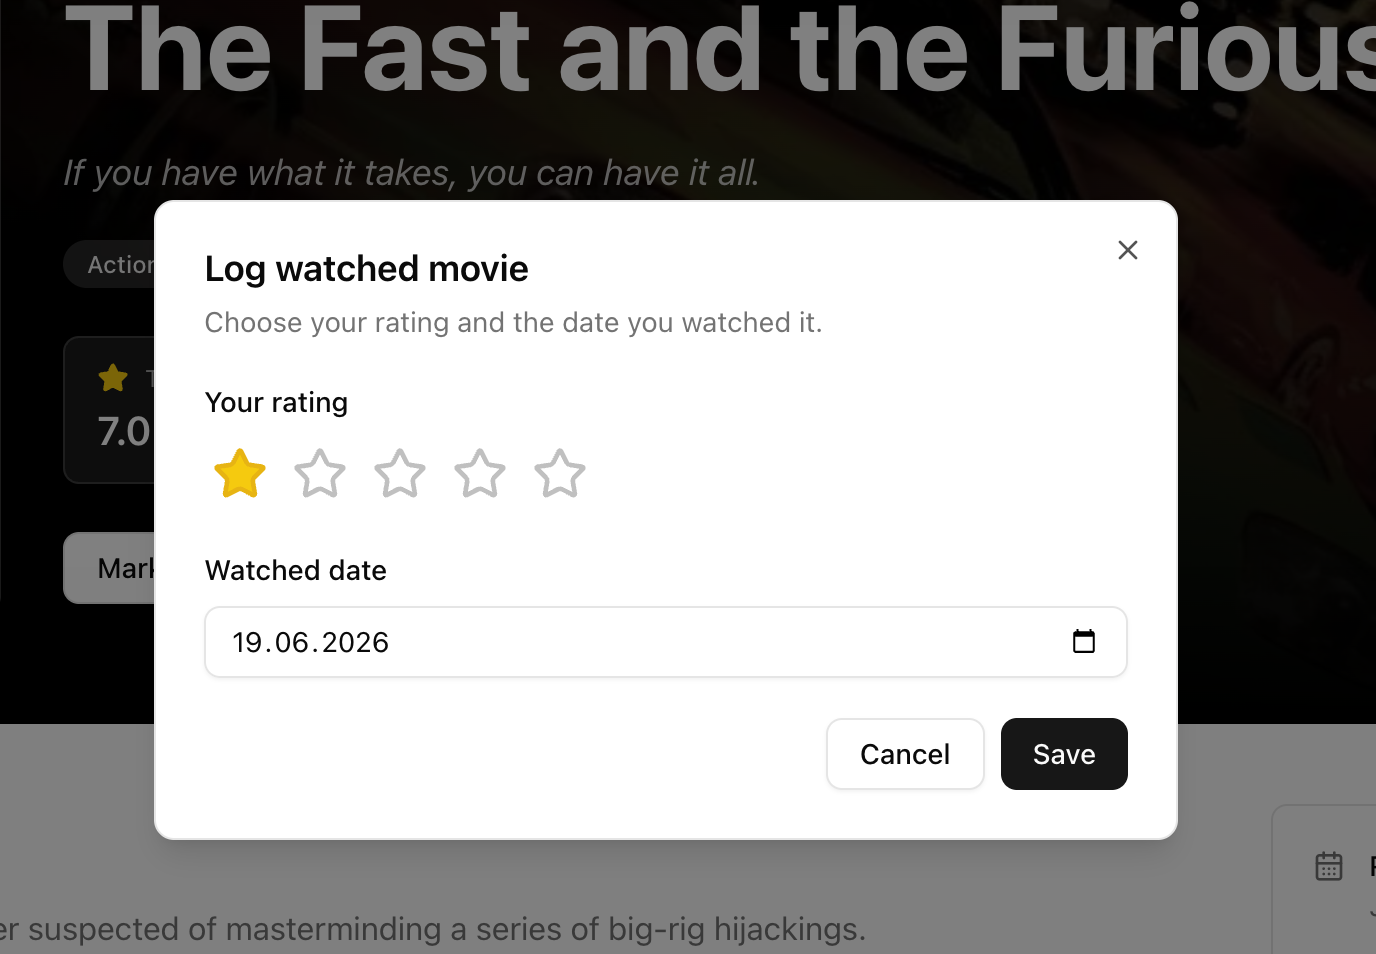
\includegraphics[width=0.58\textwidth]{chapters/chapter-6-implementation/mark-as-watched-modal.png}
    \caption{A megnézettként jelöléshez tartozó modal}
    \label{fig:watchdb-mark-as-watched-modal}
\end{figure}

A szerveroldali API route-ok minden módosítás előtt ellenőrzik az aktuális felhasználót. A watched mentésekor a rendszer validálja a film azonosítóját, az értékelést és a dátum formátumát, majd új sort hoz létre a \texttt{watched} táblában. A művelet után a film automatikusan kikerül a \texttt{watchlist} táblából, mert egy már megnézett filmnek nem szükséges továbbra is a megnézendő filmek között szerepelnie.

A kliensoldali élményt a TanStack Query cache-kezelése teszi gyorsabbá. A mutációk optimista frissítést alkalmaznak, vagyis a gombok állapota már a szerverválasz előtt frissül. Hiba esetén a korábbi állapot visszaállítható, sikeres mentés után pedig a watchlist és watched lekérdezések érvénytelenítésre kerülnek. Így a film oldal és a profiloldalon megjelenő listák ugyanazt a friss állapotot tükrözik.
